\documentclass[aspectratio=169]{beamer}
% ============================================================================
% HEC Montréal MBA -- ECON50803: Macroeconomic Environment
% Shared Beamer Preamble
% ============================================================================

% --- Theme and base settings ------------------------------------------------
\usetheme{default}
\setbeamersize{text margin left=1.2cm, text margin right=1.2cm}

% --- Fonts ------------------------------------------------------------------
% Sans-serif throughout for a business look (comment out FiraSans if unavailable)
\usepackage[sfdefault,light]{FiraSans}
\usepackage{FiraMono}
\usepackage[T1]{fontenc}
\usepackage[utf8]{inputenc}
\setbeamerfont{title}{series=\bfseries, size=\Large}
\setbeamerfont{frametitle}{series=\bfseries, size=\large}
\setbeamerfont{framesubtitle}{series=\mdseries, size=\normalsize}

% --- Colors -----------------------------------------------------------------
\definecolor{HECnavy}{HTML}{002855}
\definecolor{HECgreen}{HTML}{26d07c}
\definecolor{HECcoral}{HTML}{ff585d}
\definecolor{HECtext}{HTML}{2D3748}
\definecolor{HECgray}{HTML}{94A3B8}
\definecolor{HEClightgray}{HTML}{F1F5F9}
\definecolor{HEClightblue}{HTML}{E8EDF3}

% Beamer color assignments
\setbeamercolor{normal text}{fg=HECtext}
\setbeamercolor{title}{fg=HECnavy}
\setbeamercolor{frametitle}{fg=HECnavy}
\setbeamercolor{structure}{fg=HECnavy}
\setbeamercolor{background canvas}{bg=white}
\setbeamercolor{alerted text}{fg=HECcoral}
\setbeamercolor{example text}{fg=HECgreen}
\hypersetup{colorlinks, linkcolor=HECnavy, urlcolor=HECnavy, citecolor=HECtext}

% --- Navigation and chrome --------------------------------------------------
\setbeamertemplate{navigation symbols}{}

% Frame title: bold text with a thin accent line
\setbeamertemplate{frametitle}{%
   \vspace{0.25cm}%
   {\usebeamerfont{frametitle}\usebeamercolor[fg]{frametitle}\insertframetitle}%
   \ifx\insertframesubtitle\empty\else%
      \\[2pt]{\usebeamerfont{framesubtitle}\textcolor{HECgray}{\insertframesubtitle}}%
   \fi%
   \\[-4pt]\textcolor{HECgreen}{\rule{2.5cm}{1.5pt}}%
   \\[-2pt]%
}

% Footer: course name left, slide number right, thin rule above
\setbeamertemplate{footline}{%
   \vspace{-0.1cm}%
   \hbox to \paperwidth{%
      \hspace{1.2cm}%
      \textcolor{HEClightgray}{\rule{0.84\paperwidth}{0.4pt}}%
      \hspace{1.2cm}%
   }%
   \vspace{0.05cm}%
   \hbox to \paperwidth{%
      \hspace{1.2cm}%
      {\scriptsize\textcolor{HECgray}{ECON 50803\enspace\textbar\enspace Environnement macroéconomique}}%
      \hfill%
      {\scriptsize\textcolor{HECgray}{\insertframenumber}}%
      \hspace{1.2cm}%
   }%
   \vspace{0.15cm}%
}

% --- Itemize/enumerate styling ----------------------------------------------
\setbeamertemplate{itemize item}{\textcolor{HECnavy}{$\bullet$}}
\setbeamertemplate{itemize subitem}{\textcolor{HECgray}{$\bullet$}}
\setbeamertemplate{itemize subsubitem}{\textcolor{HECgray}{\scalebox{0.6}{$\blacktriangleright$}}}
\setbeamertemplate{enumerate item}{\textcolor{HECnavy}{\bfseries\insertenumlabel.}}
\setbeamertemplate{enumerate subitem}{\textcolor{HECgray}{\insertsubenumlabel.}}

% --- Packages ---------------------------------------------------------------
\usepackage{
   tikz, caption, subcaption, ragged2e, amsmath, bm,
   makecell, threeparttable, booktabs, mathtools,
   multirow, calc, hyperref, tabularx, colortbl,
   transparent, tcolorbox, xcolor, graphicx
}
\usepackage[round]{natbib}
\usetikzlibrary{decorations.pathreplacing, decorations.markings, calc, arrows.meta, positioning}
\usepackage[absolute,overlay]{textpos}
\captionsetup[figure]{labelformat=empty, font=small, textfont=it}
\captionsetup[table]{labelformat=empty, font=small}
\setlength{\belowcaptionskip}{0cm}
\apptocmd{\frame}{}{\justifying}

% --- Paths ------------------------------------------------------------------
\graphicspath{{../Figures/}}
\newcommand*\includetables[1]{\input{../Tables/#1.tex}}

% --- Mathematical commands --------------------------------------------------
\DeclareMathOperator*{\argmax}{arg\,max}
\newcommand{\partialof}[2]{\frac{\partial #1}{\partial #2}}
\newcommand{\totalof}[2]{\frac{\text{d}#1}{\text{d}#2}}
\newcommand{\pctchg}[1]{\%\Delta #1}
\newcommand{\smallquad}{\hspace{0.5em}}

% --- Resize equation command ------------------------------------------------
\newcommand{\resizeeq}[2]{\resizebox{#2\hsize}{!}{$#1$}}

% ============================================================================
% CUSTOM SLIDE TYPES
% ============================================================================

% --- Title slide (call with \titleframe) ------------------------------------
\newcommand{\titleframe}{%
   {\setbeamertemplate{footline}{}%
   \begin{frame}[plain]
      \begin{tikzpicture}[remember picture, overlay]
         % Navy accent bar on the left
         \fill[HECnavy] (current page.north west) rectangle
            ([xshift=0.6cm]current page.south west);
         % Green accent line
         \fill[HECgreen] ([xshift=0.6cm]current page.north west) rectangle
            ([xshift=0.65cm]current page.south west);
      \end{tikzpicture}
      \vspace{1cm}
      \hspace{0.6cm}%
      \begin{minipage}{0.85\textwidth}
         {\usebeamerfont{title}\usebeamercolor[fg]{title}\inserttitle}
         \\[12pt]
         \textcolor{HECgreen}{\rule{3cm}{2pt}}
         \\[12pt]
         {\large\textcolor{HECgray}{\insertauthor}}
         \\[6pt]
         {\normalsize\textcolor{HECgray}{\insertdate}}
      \end{minipage}
      \vfill
      \hspace{0.6cm}%
      {\footnotesize\textcolor{HECgray}{HEC Montréal \enspace\textbar\enspace MBA}}
      \vspace{0.5cm}
   \end{frame}}%
}

% --- Section divider slide --------------------------------------------------
\newcommand{\sectionframe}[1]{%
   {\setbeamertemplate{footline}{}%
   \begin{frame}[plain]
      \begin{tikzpicture}[remember picture, overlay]
         \fill[HECnavy] ([shift={(-1pt,1pt)}]current page.north west) rectangle
            ([shift={(1pt,-1pt)}]current page.south east);
         \node[anchor=center] at (current page.center) {%
            \begin{minipage}{0.8\paperwidth}
               \centering
               {\LARGE\bfseries\textcolor{white}{#1}}
               \\[12pt]
               \textcolor{HECgreen}{\rule{3cm}{2pt}}
            \end{minipage}
         };
      \end{tikzpicture}
   \end{frame}}%
}

% ============================================================================
% CUSTOM BOX ENVIRONMENTS
% ============================================================================

% Key Insight (green accent)
\newtcolorbox{keyinsight}[1][Point clé]{%
   colback=HECgreen!5,
   colframe=HECgreen,
   boxrule=0pt,
   leftrule=3pt,
   arc=8pt,
   title={\textcolor{HECgreen}{\bfseries #1}},
   coltitle=HECgreen,
   fonttitle=\bfseries,
   attach title to upper={\\[4pt]},
   left=10pt, right=10pt, top=6pt, bottom=6pt
}

% Business Implication (navy accent)
\newtcolorbox{bizimplication}[1][Implication d'affaires]{%
   colback=HECnavy!5,
   colframe=HECnavy,
   boxrule=0pt,
   leftrule=3pt,
   arc=8pt,
   title={\textcolor{HECnavy}{\bfseries #1}},
   coltitle=HECnavy,
   fonttitle=\bfseries,
   attach title to upper={\\[4pt]},
   left=10pt, right=10pt, top=6pt, bottom=6pt
}

% Warning / Important (coral accent)
\newtcolorbox{warning}[1][Important]{%
   colback=HECcoral!5,
   colframe=HECcoral,
   boxrule=0pt,
   leftrule=3pt,
   arc=8pt,
   title={\textcolor{HECcoral}{\bfseries #1}},
   coltitle=HECcoral,
   fonttitle=\bfseries,
   attach title to upper={\\[4pt]},
   left=10pt, right=10pt, top=6pt, bottom=6pt
}

% Definition (gray background)
\newtcolorbox{defbox}[1][Définition]{%
   colback=HEClightgray,
   colframe=HEClightgray,
   boxrule=0pt,
   leftrule=3pt,
   arc=8pt,
   left=10pt, right=10pt, top=6pt, bottom=6pt,
   title={\textcolor{HECnavy}{\bfseries #1}},
   coltitle=HECnavy,
   fonttitle=\bfseries,
   attach title to upper={\\[4pt]}
}

% In-Class Exercise (coral accent)
\newtcolorbox{exercise}[1][Exercice]{%
   colback=HECcoral!5,
   colframe=HECcoral,
   boxrule=0pt,
   leftrule=3pt,
   arc=8pt,
   title={\textcolor{HECcoral}{\bfseries #1}},
   coltitle=HECcoral,
   fonttitle=\bfseries,
   attach title to upper={\\[4pt]},
   left=10pt, right=10pt, top=6pt, bottom=6pt
}

% ============================================================================
% NEWSPAPER HEADLINES SLIDE TEMPLATE
% ============================================================================
% Usage: inside a frame, open a tikzpicture[remember picture, overlay], then:
%   \setcounter{newshl}{0}
%   \newsheadline{Newspaper Name}{``Headline text''}   % up to 6 entries
%   \headlinesoverlay{Large overlay text}               % optional 2nd slide
%
% Headlines are auto-positioned in a 2×3 staggered grid (left/right alternating).
%
% Logo support: place PNG files in Figures/logos/ (e.g., ft.png, economist.png).
% Use the optional argument to specify the logo file (without extension):
%   \newsheadline[ft]{Financial Times}{Headline text}   % logo + bold headline
%   \newsheadline{The Economist}{``Headline text''}      % text-only fallback

\newcounter{newshl}

\newcommand{\newsheadline}[3][]{%
   % #1 = optional logo file key (e.g., ft → logos/ft.png)
   % #2 = newspaper name (text fallback when no logo)
   % #3 = headline text
   \stepcounter{newshl}%
   \pgfmathsetmacro{\hlrow}{int((\thenewshl-1)/2)}%
   \pgfmathsetmacro{\hlcol}{int(mod(\thenewshl-1,2))}%
   \pgfmathsetmacro{\hlx}{0.8 + \hlcol * 7.8}%
   \pgfmathsetmacro{\hly}{-1.5 - \hlrow * 2.0}%
   \node[anchor=north west]
      at ([shift={(\hlx cm,\hly cm)}]current page.north west) {%
      \ifx\\#1\\%
         \begin{minipage}[t]{5.8cm}%
            \textbf{\textcolor{HECgray}{\footnotesize\MakeUppercase{#2}}}%
            \\[-1pt]%
            {\small\itshape #3}%
         \end{minipage}%
      \else%
         \begin{minipage}[c]{1.2cm}%
            \includegraphics[height=1.2cm]{logos/#1}%
         \end{minipage}%
         \hspace{6pt}%
         \begin{minipage}[c][1.2cm][c]{4.3cm}%
            \raggedright{\small\textcolor{HECtext!75}{#3}}%
         \end{minipage}%
      \fi%
   };%
}

\newcommand{\headlinesoverlay}[1]{%
   \only<2>{%
      \fill[white, opacity=0.85]
         (current page.south west) rectangle (current page.north east);%
      \node[anchor=center] at ([yshift=-0.5cm]current page.center) {%
         {\fontsize{36}{44}\selectfont\bfseries\textcolor{HECnavy}{#1}}%
      };%
   }%
}

% ============================================================================
% NAVIGATION BUTTONS (optional, for bottom-of-slide section nav)
% ============================================================================

\newlength{\buttonwidth}
\newlength{\currentxpos}
\setlength{\currentxpos}{1.2cm}
\newlength{\buttonsep}
\setlength{\buttonsep}{0.05cm}

\newcommand{\mybutton}[2]{%
   \settowidth{\buttonwidth}{#1}%
   \begin{textblock*}{\buttonwidth + 2ex}(\currentxpos, \paperheight - 2.5em)
      \hyperlink{#2}{\beamerbutton{#1}}
   \end{textblock*}%
   \addtolength{\currentxpos}{\buttonwidth + \buttonsep}%
}

% ============================================================================
% BACKUP SLIDES SUPPORT
% ============================================================================

\newcommand{\backupbegin}{%
   \newcounter{finalframe}%
   \setcounter{finalframe}{\value{framenumber}}%
}
\newcommand{\backupend}{%
   \setcounter{framenumber}{\value{finalframe}}%
}

\graphicspath{{../../Figures_EN/}}

\title{Macroeconomic language and concepts}
\author{Jean-F\'elix Brouillette}
\date{Session 1}

\begin{document}

% ============================================================================
\titleframe
% ============================================================================

% --- Slide 1: What is macroeconomics?
\begin{frame}{What is macroeconomics?}
   \textbf{Macroeconomics deals with\ldots}
   \vspace{0.15cm}
   \begin{itemize}
      \setlength\itemsep{0.2cm}
      \item Global economic phenomena: the \textbf{big picture}
      \item \textbf{Interconnections} between economic agents (e.g., consumers, firms, gov.)
      \item \textbf{Long-run} trends, \textbf{short-run} fluctuations, and economic \textbf{policy}
   \end{itemize}
   \vspace{0.4cm}
   \textbf{Macroeconomics is closely linked to many other fields:}
   \vspace{0.15cm}
   \begin{itemize}
      \setlength\itemsep{0.15cm}
      \item Politics and geopolitics
      \item Psychology and sociology
      \item Finance
      \item Environment, technology, etc.
   \end{itemize}
\end{frame}

% --- Slide 2: Macro vs. micro ---
\begin{frame}{Macroeconomics vs.\ microeconomics}
   \textbf{Microeconomics} provides great tools to study how individuals make decisions\ldots
   \\[6pt]
   \ldots but not how they \textbf{aggregate} to the economy as a whole
   \\[6pt]
   \ldots and this aggregation, in turn, matters \textbf{a lot} for individual decision-making!
   \vspace{0.5cm}

   \textbf{When individual rationality leads to collective madness\ldots}
   \vspace{0.2cm}
   \begin{itemize}
      \setlength\itemsep{0.2cm}
      \item \textbf{The paradox of thrift:} everyone saves more in a recession
      \item \textbf{Helicopter money:} too many dollars chasing too few goods
      \item \textbf{The fallacy of composition:} standing up at a hockey game
   \end{itemize}
\end{frame}

% --- Slide 3: Why should you care? (adapted from Vincent S1 slide 3) ---
\begin{frame}{Why should \textit{you} care about macroeconomics?}
   The success of any business decision rests partly on \textbf{macroeconomic conditions} \\
   \vspace{0.3cm}

   Macroeconomic events, forces, and trends\ldots
   \vspace{0.15cm}
   \begin{enumerate}
      \setlength\itemsep{0.2cm}
      \item \ldots disrupt \textbf{business strategies}
      \item \ldots influence \textbf{costs, wages, interest rates}, and \textbf{competition}
      \item \ldots are sources of \textbf{risk}, but also of \textbf{opportunity}
      \item \ldots shape \textbf{markets} on a global scale \\
   \end{enumerate}
   \vspace{0.3cm}

   \ldots and \textbf{macroeconomic jargon} will be at the heart of conversations you will have as future managers
\end{frame}

% --- Slides 4--5: Headlines collage + "Where are we now?" overlay ---
\begin{frame}{A complex and uncertain world}
   \begin{tikzpicture}[remember picture, overlay]
      \setcounter{newshl}{0}
      \newsheadline[economist]{The Economist}{``Who wrangled the best trade deal from Donald Trump?''}
      \newsheadline[bloomberg]{Bloomberg}{``Kevin Warsh’s Fed Job Already Looks Impossible''}
      \newsheadline[ft]{Financial Times}{``Gold rips past \$5,000 on fears of global turmoil''}
      \newsheadline[lapresse]{La Presse}{``Les exportations du Québec en forte baisse''}
      \newsheadline[globeandmail]{The Globe and Mail}{``Mark Carney’s speech got the world’s attention---but was it the right message?''}
      \newsheadline[wsj]{The Wall Street Journal}{``The Big Money in Today’s Economy Is Going to Capital, Not Labor''}
      \headlinesoverlay{Where are we now?}
   \end{tikzpicture}
\end{frame}

% --- Narrative arc: 6 slides after "Where are we now?" ---

% Slide N1: After a very unusual recession...
\begin{frame}{After a very unusual recession\ldots}
   \begin{figure}
      \centering
      
\includegraphics[width=0.9\textwidth]{can_unemployment.png}
   \end{figure}
\end{frame}

% Slide N2: An old enemy back from the dead...
\begin{frame}{An old enemy back from the dead\ldots}
   \begin{figure}
      \centering
      
\includegraphics[width=0.9\textwidth]{can_inflation_longrun.png}
   \end{figure}
\end{frame}

% Slide N3: A forceful response...
\begin{frame}{A forceful response\ldots}
   \begin{figure}
      \centering
      
\includegraphics[width=0.9\textwidth]{policy_rates.png}
   \end{figure}
\end{frame}

% Slide N4: A return to normal...
\begin{frame}{A return to normal\ldots}
   \begin{figure}
      \centering
      
\includegraphics[width=0.9\textwidth]{canada_inflation_recent.png}
   \end{figure}
\end{frame}

% Slide N5: Trump tariffs
\begin{frame}{The return of protectionism\ldots}
   \begin{figure}
      \centering
      
\includegraphics[width=0.9\textwidth]{us_tariff_rate.png}
   \end{figure}
\end{frame}

% Slide N6: An uncertain future...
\begin{frame}{An uncertain future\ldots}
   \begin{figure}
      \centering
      
\includegraphics[width=0.9\textwidth]{canada_employment_exports.png}
   \end{figure}
\end{frame}

% Slide N7: What about the distant future?
\begin{frame}{What about the distant future\ldots}
   \begin{figure}
      \centering
      
\includegraphics[width=0.9\textwidth]{hockey_stick_world.png}
   \end{figure}
\end{frame}

% ============================================================================
\begin{frame}{Outline}
   \begin{enumerate}
      \setlength\itemsep{0.35cm}
      \item \textbf{Course overview and logistics}
      \item Measuring the economy: GDP
      \item Comparing GDP over time
      \item Comparing GDP across countries
      \item Beyond GDP
   \end{enumerate}
\end{frame}

% ============================================================================
\sectionframe{Course overview and logistics}
% ============================================================================

\begin{frame}{Course objectives}
   \textbf{No, I will not make you economists\ldots but by the end of this course, you will:}
   \vspace{0.3cm}
   \begin{enumerate}
      \setlength\itemsep{0.3cm}
      \item Be \textbf{less intimidated} by macroeconomic discussions and jargon
      \item Be able to critically interpret \textbf{macroeconomic news} (``BS'' detector)
      \item Be aware of major \textbf{macroeconomic trends}
      \item Have \textbf{objective and coherent} conversations about macroeconomics
   \end{enumerate}
   \vspace{0.5cm}
   \begin{defbox}[What this course is \textbf{not}]
      Technical. Abstract. Ideological.
   \end{defbox}
\end{frame}

\begin{frame}{Themes to be covered}
   \begin{enumerate}
      \setlength\itemsep{0.5cm}
      \item \textbf{Long-run economic growth:} why are some countries rich and others poor?
      \item \textbf{The labor market:} inequality, technology, and AI
      \item \textbf{Business cycles:} why does the economy boom and bust?
      \item \textbf{Monetary and fiscal policy:} how governments fight recessions
      \item \textbf{International trade and imbalances:} (de)globalization, tariffs, etc.
   \end{enumerate}
\end{frame}

\begin{frame}{Teaching team}
   \begin{columns}[c]
      \begin{column}{0.35\textwidth}
         \begin{center}
            
\includegraphics[width=1.0\textwidth]{headshot}
         \end{center}
      \end{column}
      \hspace{-1cm}
      \begin{column}{0.65\textwidth}
         \textbf{Jean-F\'elix Brouillette} \\[0.15cm]
         Assistant Professor of Applied Economics \\[0.3cm]
         {\small B.B.A.\ and M.Sc.\ in Economics, HEC Montr\'eal \\
         Ph.D.\ in Economics, Stanford University} \\[0.3cm]
         \begin{itemize}
            \setlength\itemsep{0.15cm}
            \item E-mail: {\small \href{mailto:jean-felix.brouillette@hec.ca}{jean-felix.brouillette@hec.ca}}
            \item Office hours: TBD
            \item Office: 4.148 (CSC)
         \end{itemize}
      \end{column}
   \end{columns}
\end{frame}

\begin{frame}{Pedagogical material}
   \textbf{ZoneCours (ZC)}
   \vspace{0.1cm}
   \begin{itemize}
      \setlength\itemsep{0.1cm}
      \item Slides and articles posted before each class
      \item Exercises and solutions
   \end{itemize}
   \vspace{0.3cm}
   \textbf{Textbook}
   \vspace{0.1cm}
   \begin{itemize}
      \setlength\itemsep{0.1cm}
      \item Vincent \& Yared (Pearson Revel): not mandatory
      \item ZC: reference for lectures + exercises
   \end{itemize}
   \vspace{0.3cm}
   \textbf{Stay on top of macro news}
   \vspace{0.1cm}
   \begin{itemize}
      \item \textit{The Economist, The Financial Times, The Wall Street Journal, Bloomberg, La Presse Affaires, Reuters, Les Échos, etc.}
   \end{itemize}
\end{frame}

\begin{frame}{Grades}
   \vspace{0.3cm}
   \begin{tabular}{l r}
      \textbf{Team project} (two parts) & \textbf{30\%} \\[0.2cm]
      \textbf{Quiz} (session 4, $\sim$15 minutes, multiple choice) & \textbf{10\%} \\[0.2cm]
      \textbf{Final exam} (March 30th) & \textbf{50\%} \\[0.2cm]
      \textbf{Contribution and professionalism} & \textbf{10\%} \\
   \end{tabular}
   \vspace{0.4cm}
   \begin{defbox}[Details]
      Team project details are on ZC. Examples of quiz questions will be provided.
   \end{defbox}
\end{frame}

\begin{frame}{Contribution and professionalism}
   \small
   \textbf{Criteria:}
   \vspace{0.15cm}
   \begin{enumerate}
      \setlength\itemsep{0.2cm}
      \item \textbf{Attendance and punctuality} --- as per program requirements
      \item \textbf{Active participation} --- quality and relevance of interventions
      \item \textbf{Professionalism} --- autonomy, judgment, collegiality
   \end{enumerate}
   \vspace{0.4cm}
   \textbf{To promote active learning:}
   \vspace{0.15cm}
   \begin{enumerate}
      \setlength\itemsep{0.2cm}
      \item \textbf{Name cards} --- please bring yours to every class
      \item \textbf{No laptops} in class (exception: tablets lying flat)
      \item \textbf{Limit comings and goings} during class
   \end{enumerate}
\end{frame}

% ============================================================================
\begin{frame}{Outline}
   \begin{enumerate}
      \setlength\itemsep{0.35cm}
      \item {\color{gray!50}Course overview and logistics}
      \item \textbf{Measuring the economy: GDP}
      \item Comparing GDP over time
      \item Comparing GDP across countries
      \item Beyond GDP
   \end{enumerate}
\end{frame}

% ============================================================================
\sectionframe{Measuring the economy: GDP}
% ============================================================================

\begin{frame}{What is GDP?}
   \begin{defbox}[Gross Domestic Product (GDP)]
      The total \textbf{market value} of all \textbf{final} goods and services produced \textbf{within a country} during a \textbf{given period}.
   \end{defbox}
   \vspace{0.3cm}
   \textbf{Key words:}
   \vspace{0.15cm}
   \begin{itemize}
      \setlength\itemsep{0.15cm}
      \item \textbf{Market value:} measured in dollars (or another currency)
      \item \textbf{Final:} excludes intermediate goods to avoid double-counting
      \item \textbf{Within a country:} production on Canadian soil
      \item \textbf{Given period:} a flow, not a stock (typically quarterly or annual)
   \end{itemize}
\end{frame}

\begin{frame}[t]{Three ways to measure GDP}
   \framesubtitle{They all give the same answer}

   \small
   \noindent%
   \begin{minipage}[t]{0.33\textwidth}
      \textbf{\textcolor{HECnavy}{1. Expenditure}}\\[4pt]
      Who is buying?
      \vspace{-0.2cm}
      \begin{equation*}
         Y = C + I + G + NX
      \end{equation*}
      \vspace{-0.8cm}
      \begin{itemize}
         \footnotesize
         \item $C$: consumption
         \item $I$: investment
         \item $G$: gov. spending
         \item $NX$: net exports
      \end{itemize}
   \end{minipage}%
   \begin{minipage}[t]{0.33\textwidth}
      \textbf{\textcolor{HECnavy}{2. Income}}\\[4pt]
      Who is earning?
      \vspace{0.1cm}
      \begin{itemize}
         \footnotesize
         \item Wages/salaries
         \item Corporate profits
         \item Rental income
         \item Interest income
      \end{itemize}
   \end{minipage}%
   \hspace{-0.5cm}
   \begin{minipage}[t]{0.33\textwidth}
      \textbf{\textcolor{HECnavy}{3. Value added}}\\[4pt]
      Who is producing?
      \vspace{0.1cm}
      \begin{itemize}
         \footnotesize
         \item Value added at each stage
         \item Revenue $-$ int. inputs
      \end{itemize}
   \end{minipage}
   \vspace{0.1cm}
   \begin{keyinsight}
      Every dollar spent is a dollar earned is a dollar of value created
   \end{keyinsight}
\end{frame}

\begin{frame}[t]{Example: value added avoids double counting}
   \footnotesize
   \begin{tcolorbox}[
      colback=white, colframe=HECnavy, colbacktitle=HECnavy,
      title=\textbf{Example}, fonttitle=\footnotesize, boxrule=0.5pt, arc=8pt,
      top=3pt, bottom=3pt, left=6pt, right=6pt
   ]
      A business hires employees to work in a fertilizer plant and pays them \$0.50 in wages. The business sells the fertilizer to Dwight, a self-employed farmer, for \$0.80. Dwight uses it to produce beets, which he sells to Jim for \$1. Jim eats the beets.
      \vspace{0.1cm}

      \renewcommand{\arraystretch}{1.1}
      \centering
      \begin{tabularx}{\linewidth}{X r >{\hspace{0.15cm}}X r >{\hspace{0.15cm}}X r}
         \rowcolor{HECnavy!10}
         \textbf{Production} & & \textbf{Income} & & \textbf{Expenditure} & \\
         \hline
         Manufacturing & 0.80 & Wages & 0.50 & Consumption & 1.00 \\
         Agriculture & 0.20 & Profits & 0.30 & & \\
         & & Prop.\ income & 0.20 & & \\
         \hline
         \textbf{Total} & \textbf{1.00} & \textbf{Total} & \textbf{1.00} & \textbf{Total} & \textbf{1.00}
      \end{tabularx}
   \end{tcolorbox}
   \vspace{0.05cm}
   \begin{keyinsight}
      Production = \textbf{value added} (revenue $-$ intermediate inputs), not total revenue. This avoids double counting and ensures all three approaches agree.
   \end{keyinsight}
\end{frame}

\begin{frame}{The expenditure approach: $Y = C + I + G + NX$}
   \begin{figure}
      \centering
      
\includegraphics[height=0.8\textheight]{gdp_decomposition_canada.png}
   \end{figure}
\end{frame}

% ── Consumption ───────────────────────────────────────────────────────

\begin{frame}[t]{Consumption ($C$)}
   \textbf{Household spending} on final goods and services:
   \vspace{0.2cm}
   \begin{itemize}
      \setlength\itemsep{0.15cm}
      \item \textbf{Durable goods} --- cars, furniture, appliances (long-lasting)
      \item \textbf{Non-durable goods} --- food, clothing, gasoline (used up quickly)
      \item \textbf{Services} --- rent, healthcare, haircuts, education
   \end{itemize}
   \vspace{0.3cm}
   \begin{keyinsight}
      Services account for over 60\% of consumption in Canada. The shift from goods to services is a hallmark of advanced economies.
   \end{keyinsight}
\end{frame}

\begin{frame}{Consumption share of GDP in Canada}
   \vspace{-0.2cm}
   \begin{figure}
      \centering
      
\includegraphics[width=0.95\textwidth]{consumption_share_gdp.png}
   \end{figure}
   \vspace{-0.4cm}
   \footnotesize Consumption is the largest component ($\approx$60\%), and increasing over time.
\end{frame}

% ── Investment ────────────────────────────────────────────────────────

\begin{frame}[t]{Investment ($I$)}
   \textbf{Spending on goods used to produce future output:}
   \vspace{0.2cm}
   \begin{itemize}
      \setlength\itemsep{0.15cm}
      \item \textbf{Business fixed capital} --- machines, equipment, factories, software
      \item \textbf{Residential} --- new housing construction
      \item \textbf{Inventories} --- unsold goods stored in warehouses
   \end{itemize}
   \vspace{0.3cm}
   \begin{warning}[Common confusion]
      In economics, ``investment'' means \textbf{physical capital formation}, not buying stocks or bonds. A firm purchasing a delivery van is investment; buying shares of Tesla is not.
   \end{warning}
\end{frame}

\begin{frame}[t]{Example: investment}
   \footnotesize
   \begin{tcolorbox}[
      colback=white, colframe=HECnavy, colbacktitle=HECnavy,
      title=\textbf{Example}, fonttitle=\footnotesize, boxrule=0.5pt, arc=8pt,
      top=3pt, bottom=3pt, left=6pt, right=6pt
   ]
      General Motors produces a minivan, which it sells for \$1,000 to the Michael Scott Paper Company. The cost of producing it is made up of workers' wages worth \$600.
      \vspace{0.1cm}

      \renewcommand{\arraystretch}{1.1}
      \centering
      \begin{tabularx}{\linewidth}{X r >{\hspace{0.15cm}}X r >{\hspace{0.15cm}}X r}
         \rowcolor{HECnavy!10}
         \textbf{Production} & & \textbf{Income} & & \textbf{Expenditure} & \\
         \hline
         Manufacturing & 1,000 & Wages & 600 & Investment & 1,000 \\
         & & Profits & 400 & & \\
         \hline
         \textbf{Total} & \textbf{1,000} & \textbf{Total} & \textbf{1,000} & \textbf{Total} & \textbf{1,000}
      \end{tabularx}
   \end{tcolorbox}
   \vspace{0.05cm}
   \begin{keyinsight}
      A firm buying a capital good = \textbf{investment}, not consumption.
   \end{keyinsight}
\end{frame}

\begin{frame}[t]{Example: inventories (Year 1)}
   \footnotesize
   \begin{tcolorbox}[
      colback=white, colframe=HECnavy, colbacktitle=HECnavy,
      title=\textbf{Example}, fonttitle=\footnotesize, boxrule=0.5pt, arc=8pt,
      top=3pt, bottom=3pt, left=6pt, right=6pt
   ]
      Dunder Mifflin produces 500 tons of white paper worth \$400 and stores them in its warehouse while it waits for customers to buy them. The cost of producing them is made up of workers' wages of \$500.
      \vspace{0.1cm}

      \renewcommand{\arraystretch}{1.1}
      \centering
      \begin{tabularx}{\linewidth}{X r >{\hspace{0.15cm}}X r >{\hspace{0.15cm}}X r}
         \rowcolor{HECnavy!10}
         \textbf{Production} & & \textbf{Income} & & \textbf{Expenditure} & \\
         \hline
         Manufacturing & 400 & Wages & 500 & Investment & 400 \\
         & & Profits & (100) & & \\
         \hline
         \textbf{Total} & \textbf{400} & \textbf{Total} & \textbf{400} & \textbf{Total} & \textbf{400}
      \end{tabularx}
   \end{tcolorbox}
   \vspace{0.05cm}
   \begin{keyinsight}
      Unsold goods = \textbf{inventory investment}. GDP captures all production, even without a sale.
   \end{keyinsight}
\end{frame}

\begin{frame}[t]{Example: inventories (Year 2)}
   \footnotesize
   \begin{tcolorbox}[
      colback=white, colframe=HECnavy, colbacktitle=HECnavy,
      title=\textbf{Example}, fonttitle=\footnotesize, boxrule=0.5pt, arc=8pt,
      top=3pt, bottom=3pt, left=6pt, right=6pt
   ]
      The following year, Dunder Mifflin finally sells its paper worth \$400.
      \vspace{0.1cm}

      \renewcommand{\arraystretch}{1.1}
      \centering
      \begin{tabularx}{\linewidth}{X r >{\hspace{0.15cm}}X r >{\hspace{0.15cm}}X r}
         \rowcolor{HECnavy!10}
         \textbf{Production} & & \textbf{Income} & & \textbf{Expenditure} & \\
         \hline
         & & & & Consumption & 400 \\
         & & & & Investment & (400) \\
         \hline
         \textbf{Total} & \textbf{0} & \textbf{Total} & \textbf{0} & \textbf{Total} & \textbf{0}
      \end{tabularx}
   \end{tcolorbox}
   \vspace{0.05cm}
   \begin{keyinsight}
      Selling from inventory: $C$ rises, $I$ falls $\Rightarrow$ GDP = 0. Production was counted in year~1.
   \end{keyinsight}
\end{frame}

\begin{frame}{Investment share of GDP in Canada}
   \vspace{-0.2cm}
   \begin{figure}
      \centering
      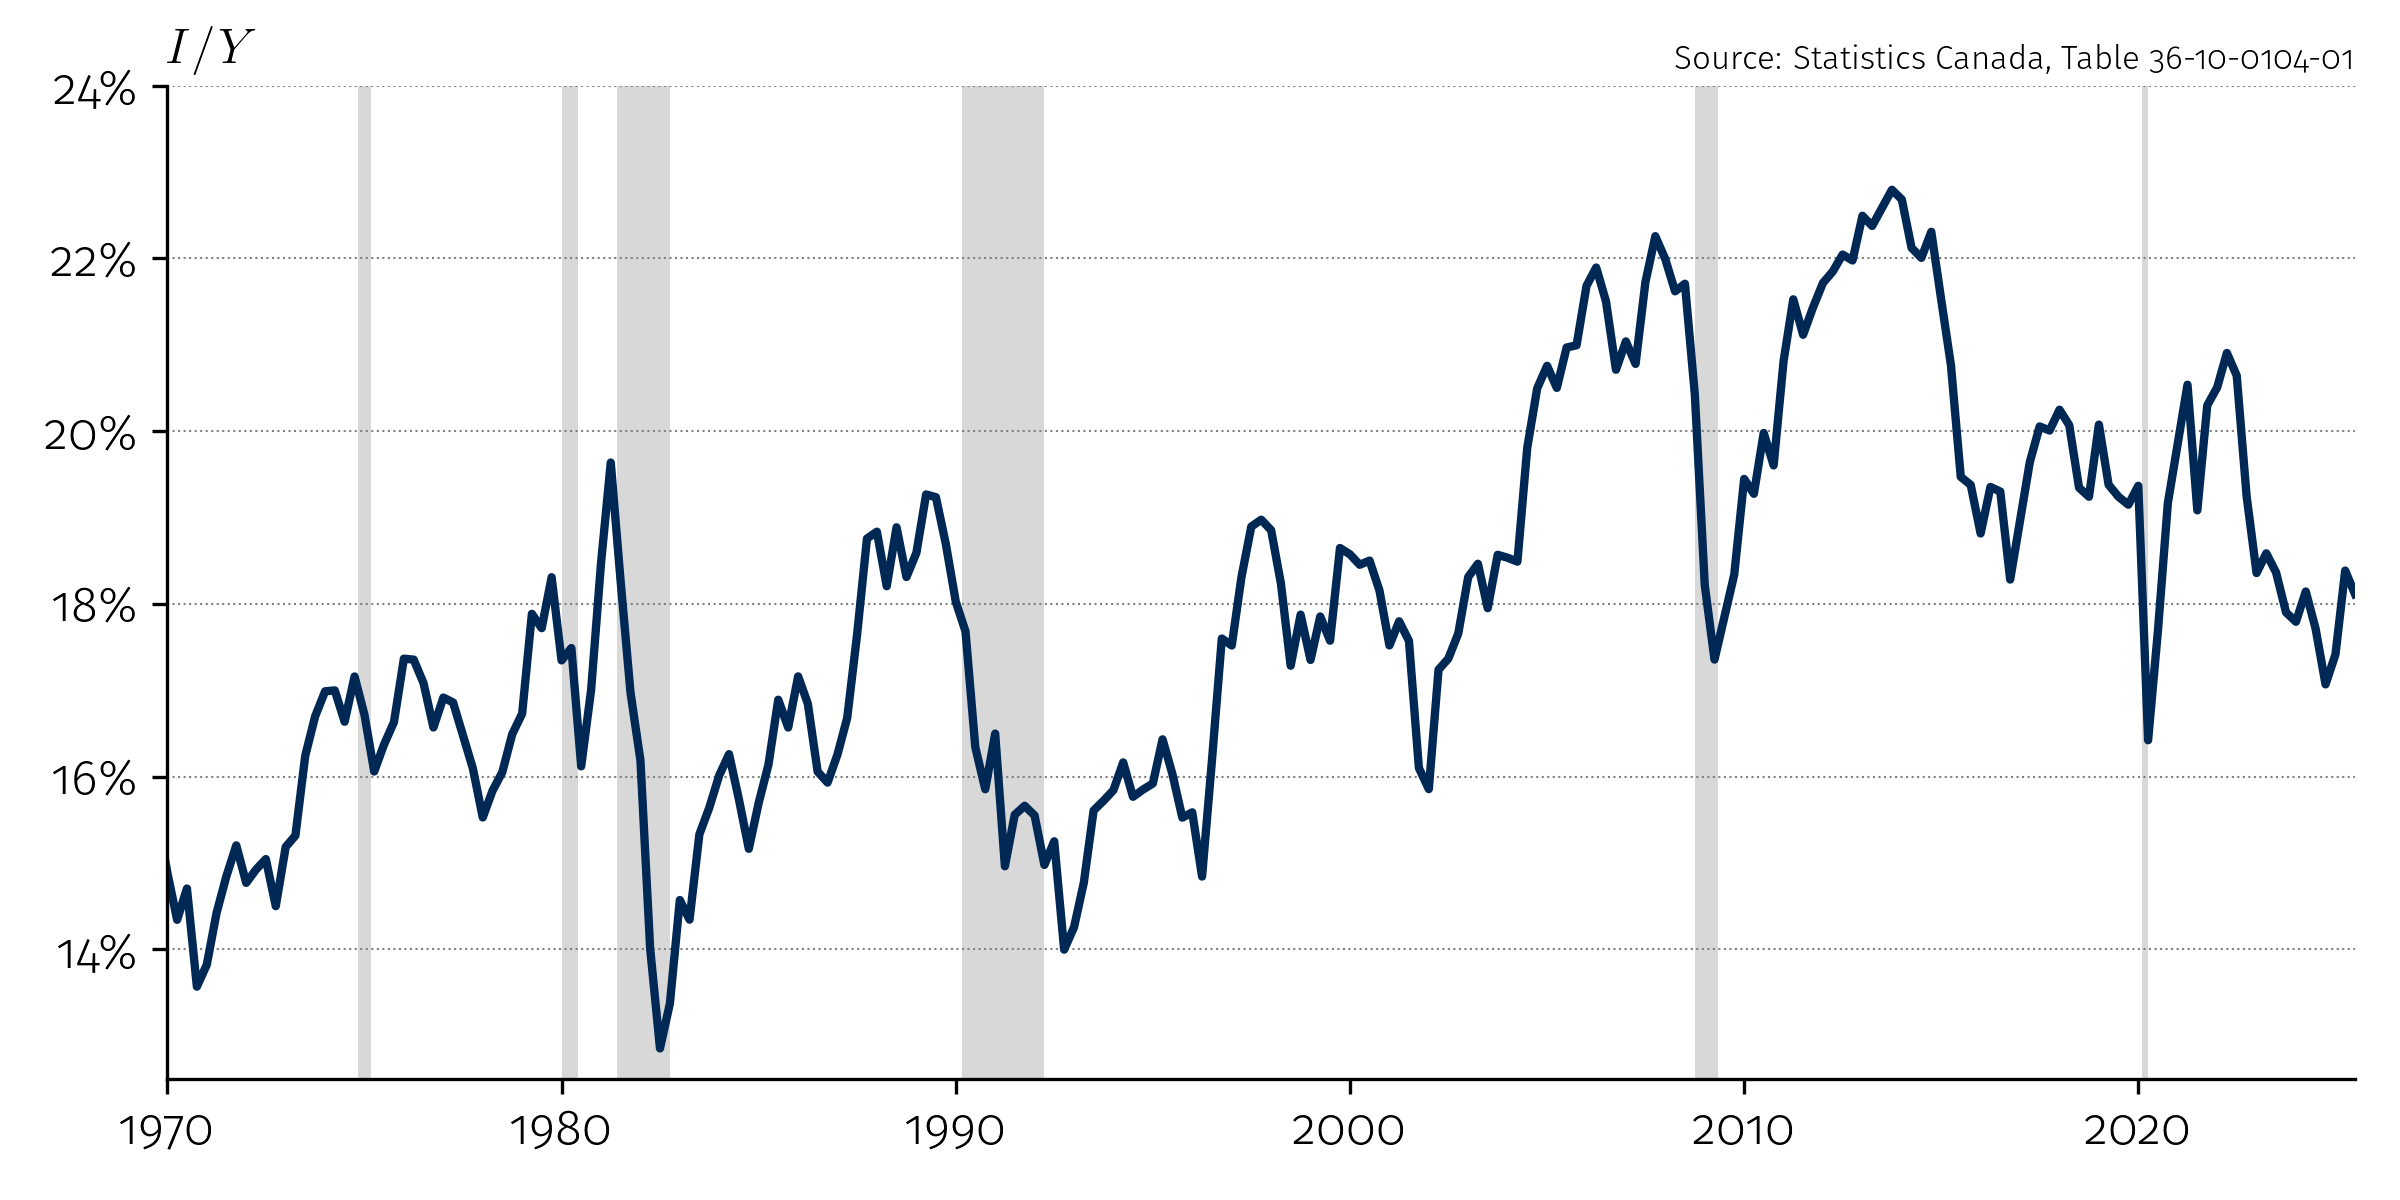
\includegraphics[width=0.95\textwidth]{investment_share_gdp.png}
   \end{figure}
   \vspace{-0.4cm}
   \footnotesize Investment is the most \textbf{volatile} component --- it swings sharply during recessions.
\end{frame}

% ── Government spending ───────────────────────────────────────────────

\begin{frame}[t]{Government spending ($G$)}
   \small
   \textbf{Major producer} of goods/services:
   military, education, healthcare, infrastructure.
   \vspace{0.15cm}
   \begin{defbox}[Valued at cost]
      Often missing market prices, so $G$ measured using \textbf{cost of inputs}.
   \end{defbox}
   \vspace{0.1cm}
   \begin{warning}[Transfers $\neq$ government spending]
      Social transfers (UI, pensions, welfare) are \textbf{not} in $G$ because they do not involve any new production --- they redistribute existing income.
   \end{warning}
\end{frame}

\begin{frame}{Government spending share of GDP in Canada}
   \vspace{-0.2cm}
   \begin{figure}
      \centering
      
\includegraphics[width=0.95\textwidth]{government_share_gdp.png}
   \end{figure}
   \vspace{-0.4cm}
   \footnotesize Government spending spikes in recessions, but on a long downward trend since the 1990s.
\end{frame}

% ── Exports and imports ───────────────────────────────────────────────

\begin{frame}[t]{Exports and imports ($NX$)}
   $C$, $I$, and $G$ include spending on \textbf{foreign} goods (imports).\\[4pt]
   Since GDP measures \textit{domestic} production, we need a correction:
   \vspace{0.1cm}
   \begin{equation*}
      Y = \underbrace{C + I + G}_{\text{total spending}} + \underbrace{X - M}_{\text{net exports}}
   \end{equation*}
   \vspace{-0.3cm}
   \begin{itemize}
      \setlength\itemsep{0.1cm}
      \item $X$ (exports): domestic production sold to foreigners
      \item $M$ (imports): foreign production already counted in $C$, $I$, $G$
   \end{itemize}
   \vspace{0.15cm}
   \begin{defbox}[Trade openness]
      $(X + M) / Y$ measures how important trade is for an economy.
   \end{defbox}
\end{frame}

\begin{frame}{Trade share of GDP in Canada}
   \vspace{-0.2cm}
   \begin{figure}
      \centering
      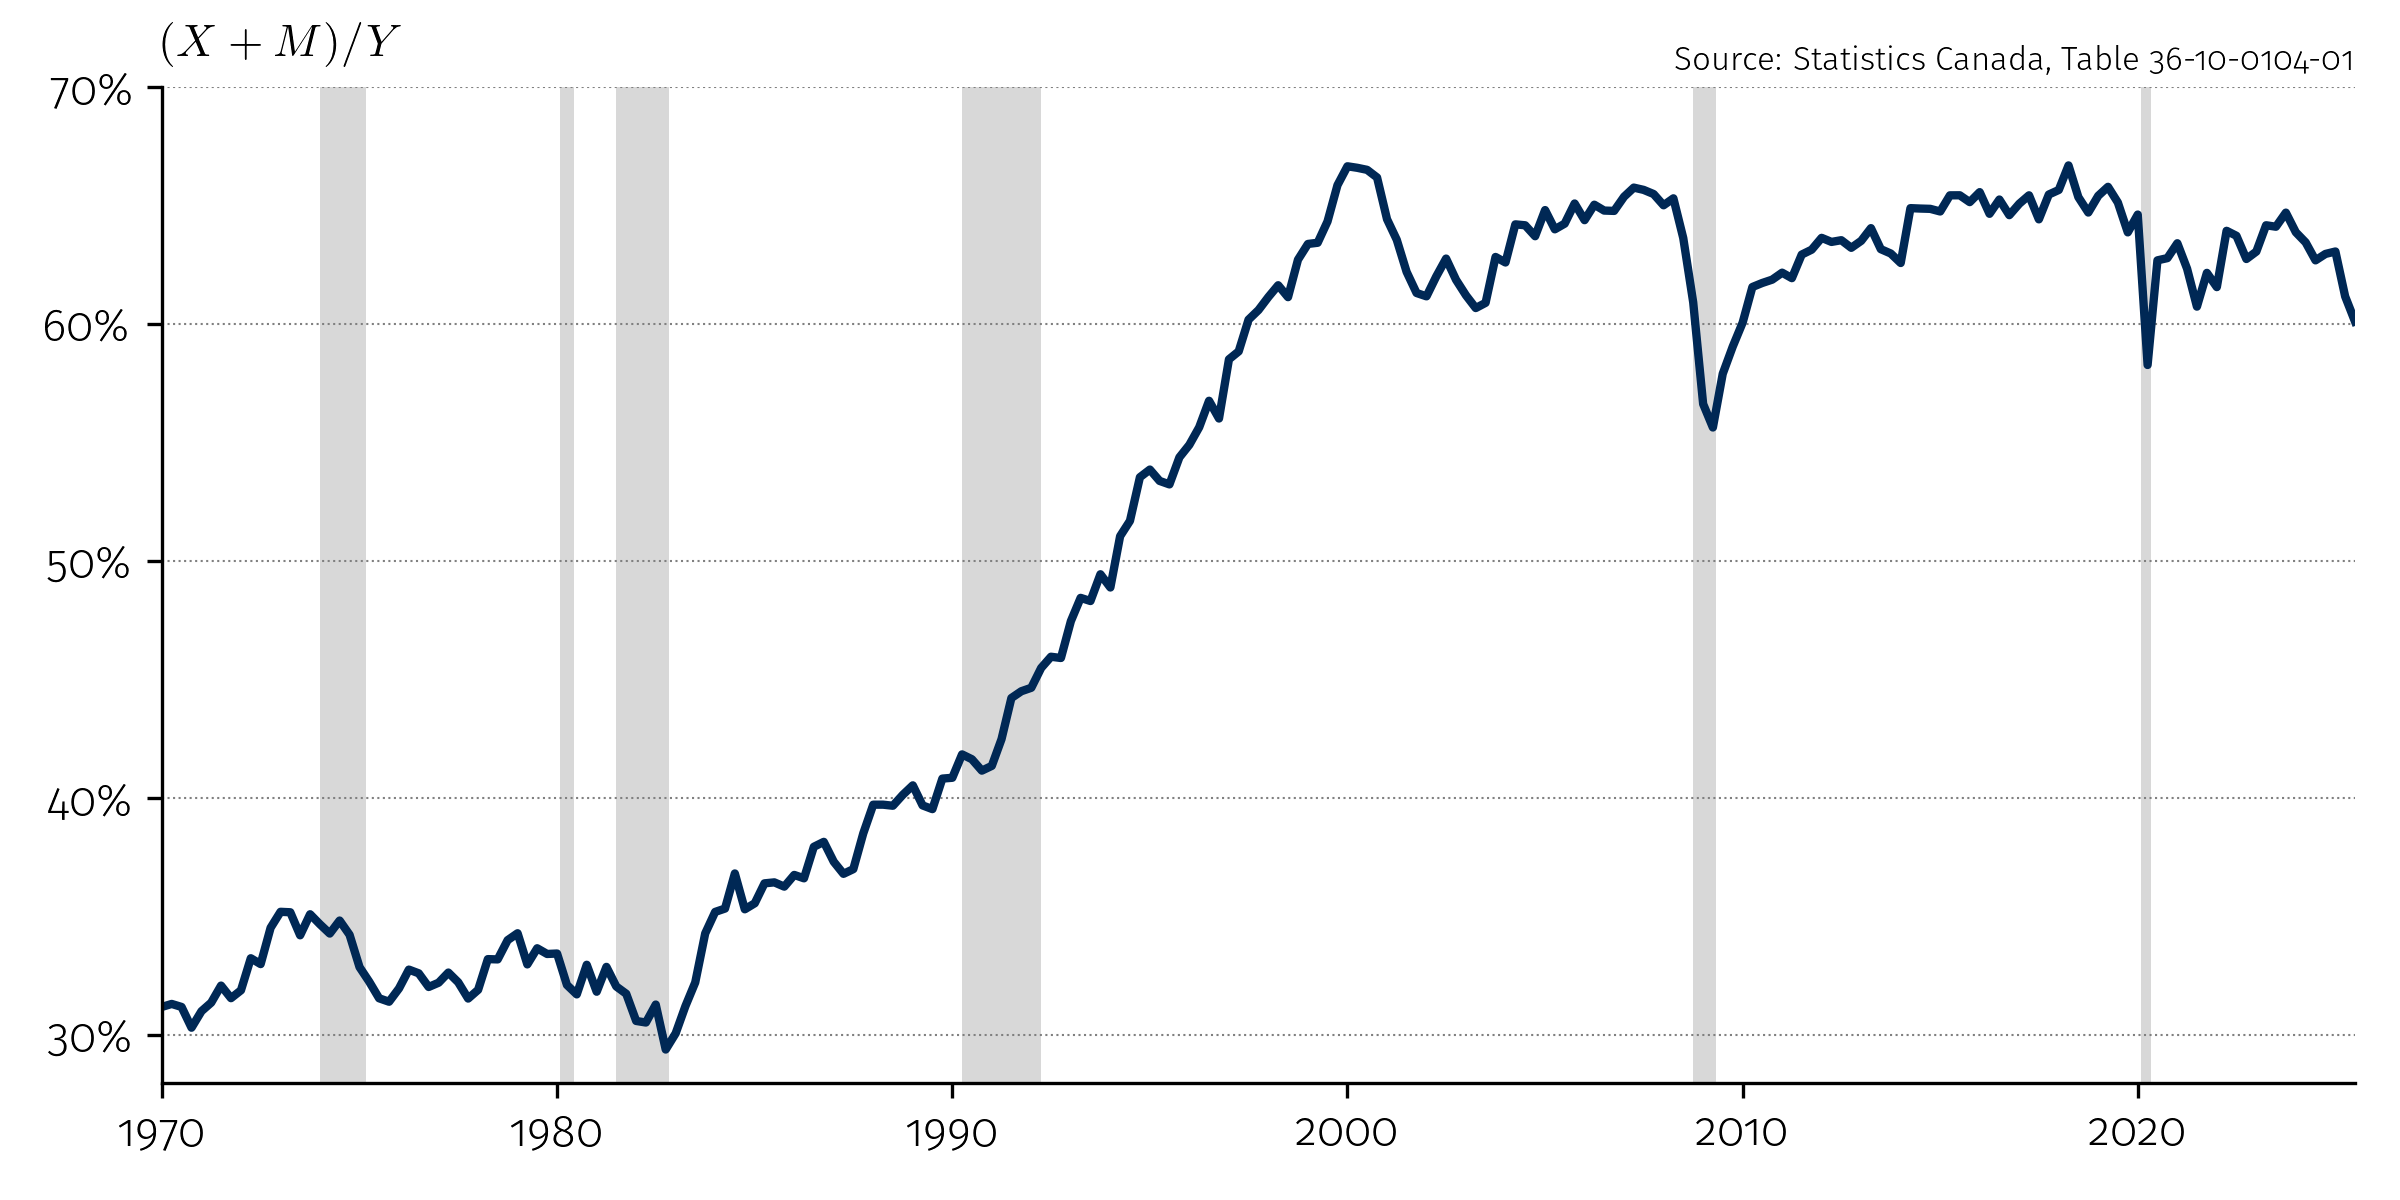
\includegraphics[width=0.95\textwidth]{trade_share_gdp.png}
   \end{figure}
   \vspace{-0.4cm}
   \footnotesize Canada is a very open economy. Trade peaked with NAFTA (1994) and has slightly declined since.
\end{frame}

\begin{frame}[t]{Training your ``BS'' detector}
   \footnotesize
   \vspace{0.1cm}
   \begin{columns}[T]
      \begin{column}{0.42\textwidth}
         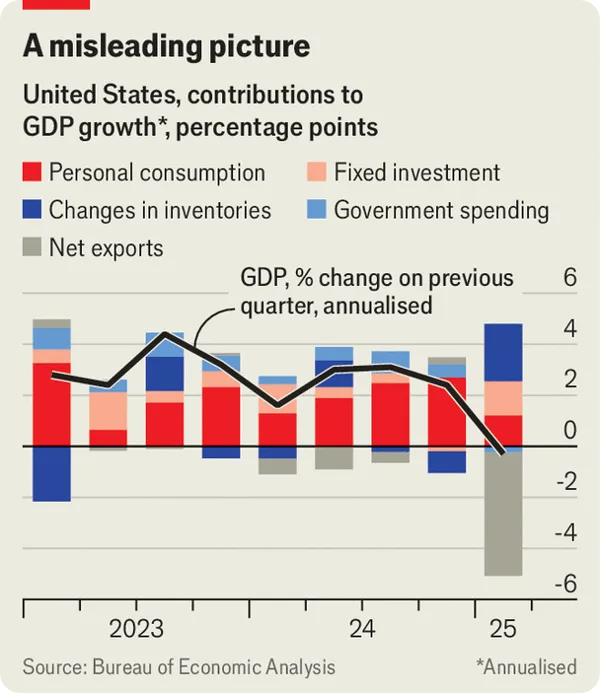
\includegraphics[width=\linewidth, height=0.65\textheight, keepaspectratio]{misleading_GDP_accounting.png}\\[-2pt]
         {\scriptsize\textcolor{HECgray}{Source: \textit{The Economist}, 2025}}
      \end{column}
      \hspace{-2cm}
      \begin{column}{0.54\textwidth}
         In Q1 2025, US GDP fell. Many blamed imports: ``the trade deficit subtracted 5~pp from GDP growth.''
         \vspace{0.15cm}
         \begin{warning}[That's misleading]
            \footnotesize
            Imports enter GDP \textbf{twice}: once \textit{added} in $C$, $I$, or $G$, and once \textit{subtracted} in $NX$.\\[8pt]
            If firms front-load imports before tariffs, inventories surge ($\uparrow I$) while net exports plunge ($\downarrow NX$). The two cancel out.\\[8pt]
            If consumers hurry to buy dishwashers before tariffs, consumption surges ($\uparrow C$) while net exports plunge ($\downarrow NX$). The two cancel out.
         \end{warning}
      \end{column}
   \end{columns}
\end{frame}

\begin{frame}{GDP by expenditure: cross-country comparison}
   \begin{figure}
      \centering
      
\includegraphics[width=\textwidth]{gdp_decomposition_4countries.png}
   \end{figure}
   \vspace{-0.2cm}
   \begin{keyinsight}[Different growth models]
      China is investment-driven ($I$ = 41\%), while the US is consumption-driven ($C$ = 68\%). These differences shape trade patterns and growth strategies.
   \end{keyinsight}
\end{frame}

\begin{frame}[t]{What GDP does \textit{not} measure}
   GDP only counts \textbf{market transactions}. A lot of economic activity is missed:
   \vspace{0.2cm}
   \begin{itemize}
      \setlength\itemsep{0.15cm}
      \item \textbf{Household production} --- cooking, childcare, home repairs
      \item \textbf{Volunteer work} --- community services, charities
      \item \textbf{Underground economy} --- unreported income, informal work
   \end{itemize}
   \vspace{0.2cm}
   \begin{keyinsight}[Sex, drugs, and GDP]
      In 2014, EU accounting rules began requiring countries to include estimates of illegal activities (e.g., drugs, prostitution) in GDP. Italy's GDP rose by 18\% overnight\ldots
      \hfill{\scriptsize\textit{\color{black!50}The Economist, 2014}}
   \end{keyinsight}
\end{frame}

\begin{frame}{Can we trust GDP figures?}
   \centering
   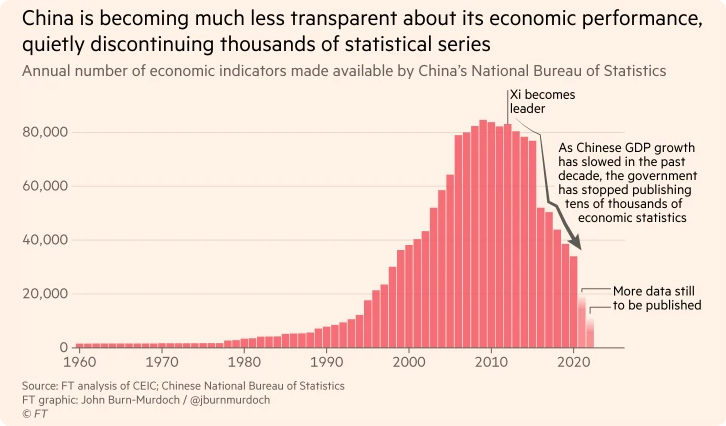
\includegraphics[height=0.75\textheight, keepaspectratio]{china_transparency.png}
\end{frame}

\begin{frame}[t]{GDP manipulation: three cautionary tales}
   \small
   \begin{itemize}
      \setlength\itemsep{0.1cm}
      \item \textbf{China:} Suspiciously smooth GDP growth, statistical series are increasingly discontinued, and provinces routinely report figures matching central targets\ldots Autocracies overstate growth by $\sim$35\% on average.
         \\{\scriptsize\textcolor{HECgray}{Martinez, ``How Much Should We Trust the Dictator's GDP Growth Estimates?'' \textit{JPE}, 2022}}
      \item \textbf{Venezuela:} the central bank stopped publishing GDP and inflation data from 2016 to 2019; when it resumed, it revealed a cumulative GDP contraction of $\sim$47\%
         \\{\scriptsize\textcolor{HECgray}{IMF World Economic Outlook; Banco Central de Venezuela, 2019}}
      \item \textbf{Greece:} the 2009 deficit was reported as 3.7\% of GDP, then revised to 15.4\% --- more than four times the original figure, triggering the eurozone debt crisis
         \\{\scriptsize\textcolor{HECgray}{European Commission, Report on Greek Government Deficit and Debt Statistics, 2010}}
   \end{itemize}
   \begin{bizimplication}[Due diligence]
      \footnotesize When evaluating market entry or investment, don't take official GDP at face value. Cross-check with alternative data --- especially in autocracies.
   \end{bizimplication}
\end{frame}

\begin{frame}[t]{When data goes missing\ldots economists get creative!}
   \footnotesize
   \begin{itemize}
      \setlength\itemsep{0.3cm}
      \item \textbf{Satellite night lights:} brightness correlates with economic activity --- for poor-data countries, night lights are as informative as official GDP,
         {\scriptsize\textcolor{HECgray}{(Henderson et al., \textit{AER}, 2012).}}
      \item \textbf{Trade and port data:} shipping volumes, ship AIS draft depth, customs records, and container throughput reveal trade flows that official statistics may undercount.
      \item \textbf{ML inference:} ML algorithms detect oil tankers turning off transponders to evade sanctions (dark shipping), mapping illicit trade flows in real time,
         {\scriptsize\textcolor{HECgray}{(Fern\'andez-Villaverde et al., NBER WP 33486, 2025).}}
      \item \textbf{Online prices:} web-scraped retail prices track inflation daily --- famously exposed Argentina's manipulated CPI,
         {\scriptsize\textcolor{HECgray}{(Cavallo \& Rigobon, \textit{JEP}, 2016).}}
      \item \textbf{Mobile phone data:} call density and airtime purchases proxy for consumption in developing countries.
   \end{itemize}
\end{frame}

\begin{frame}{When darkness sheds light\ldots}
   \centering
   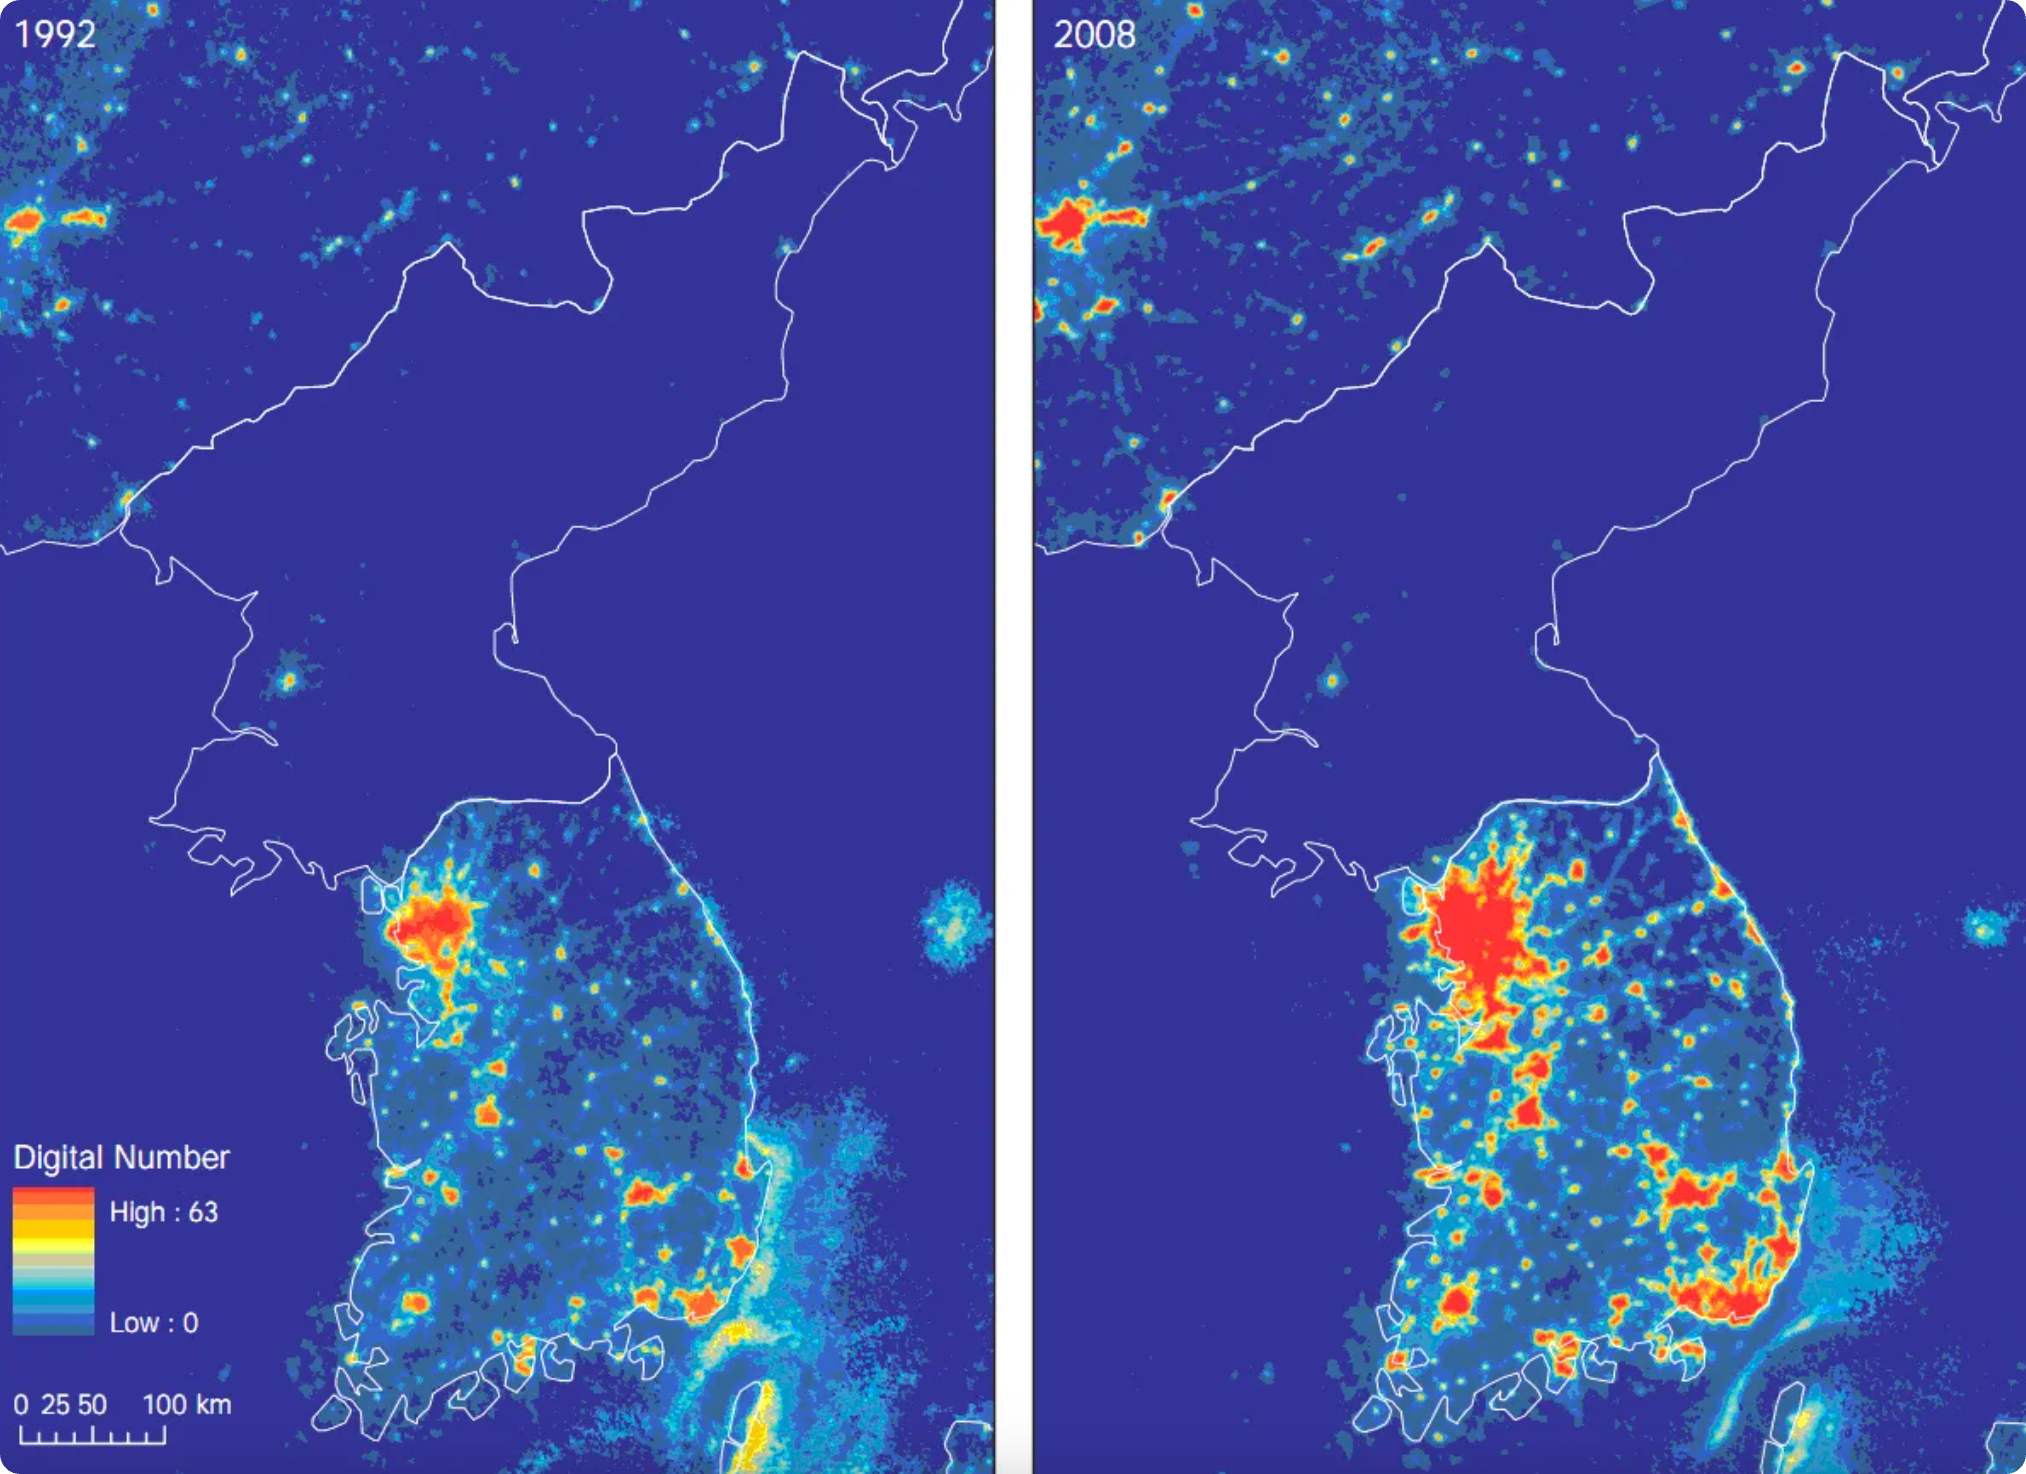
\includegraphics[height=0.75\textheight, keepaspectratio]{korea_space.png}
\end{frame}

\begin{frame}[t]{When darkness sheds light\ldots}
   \centering
   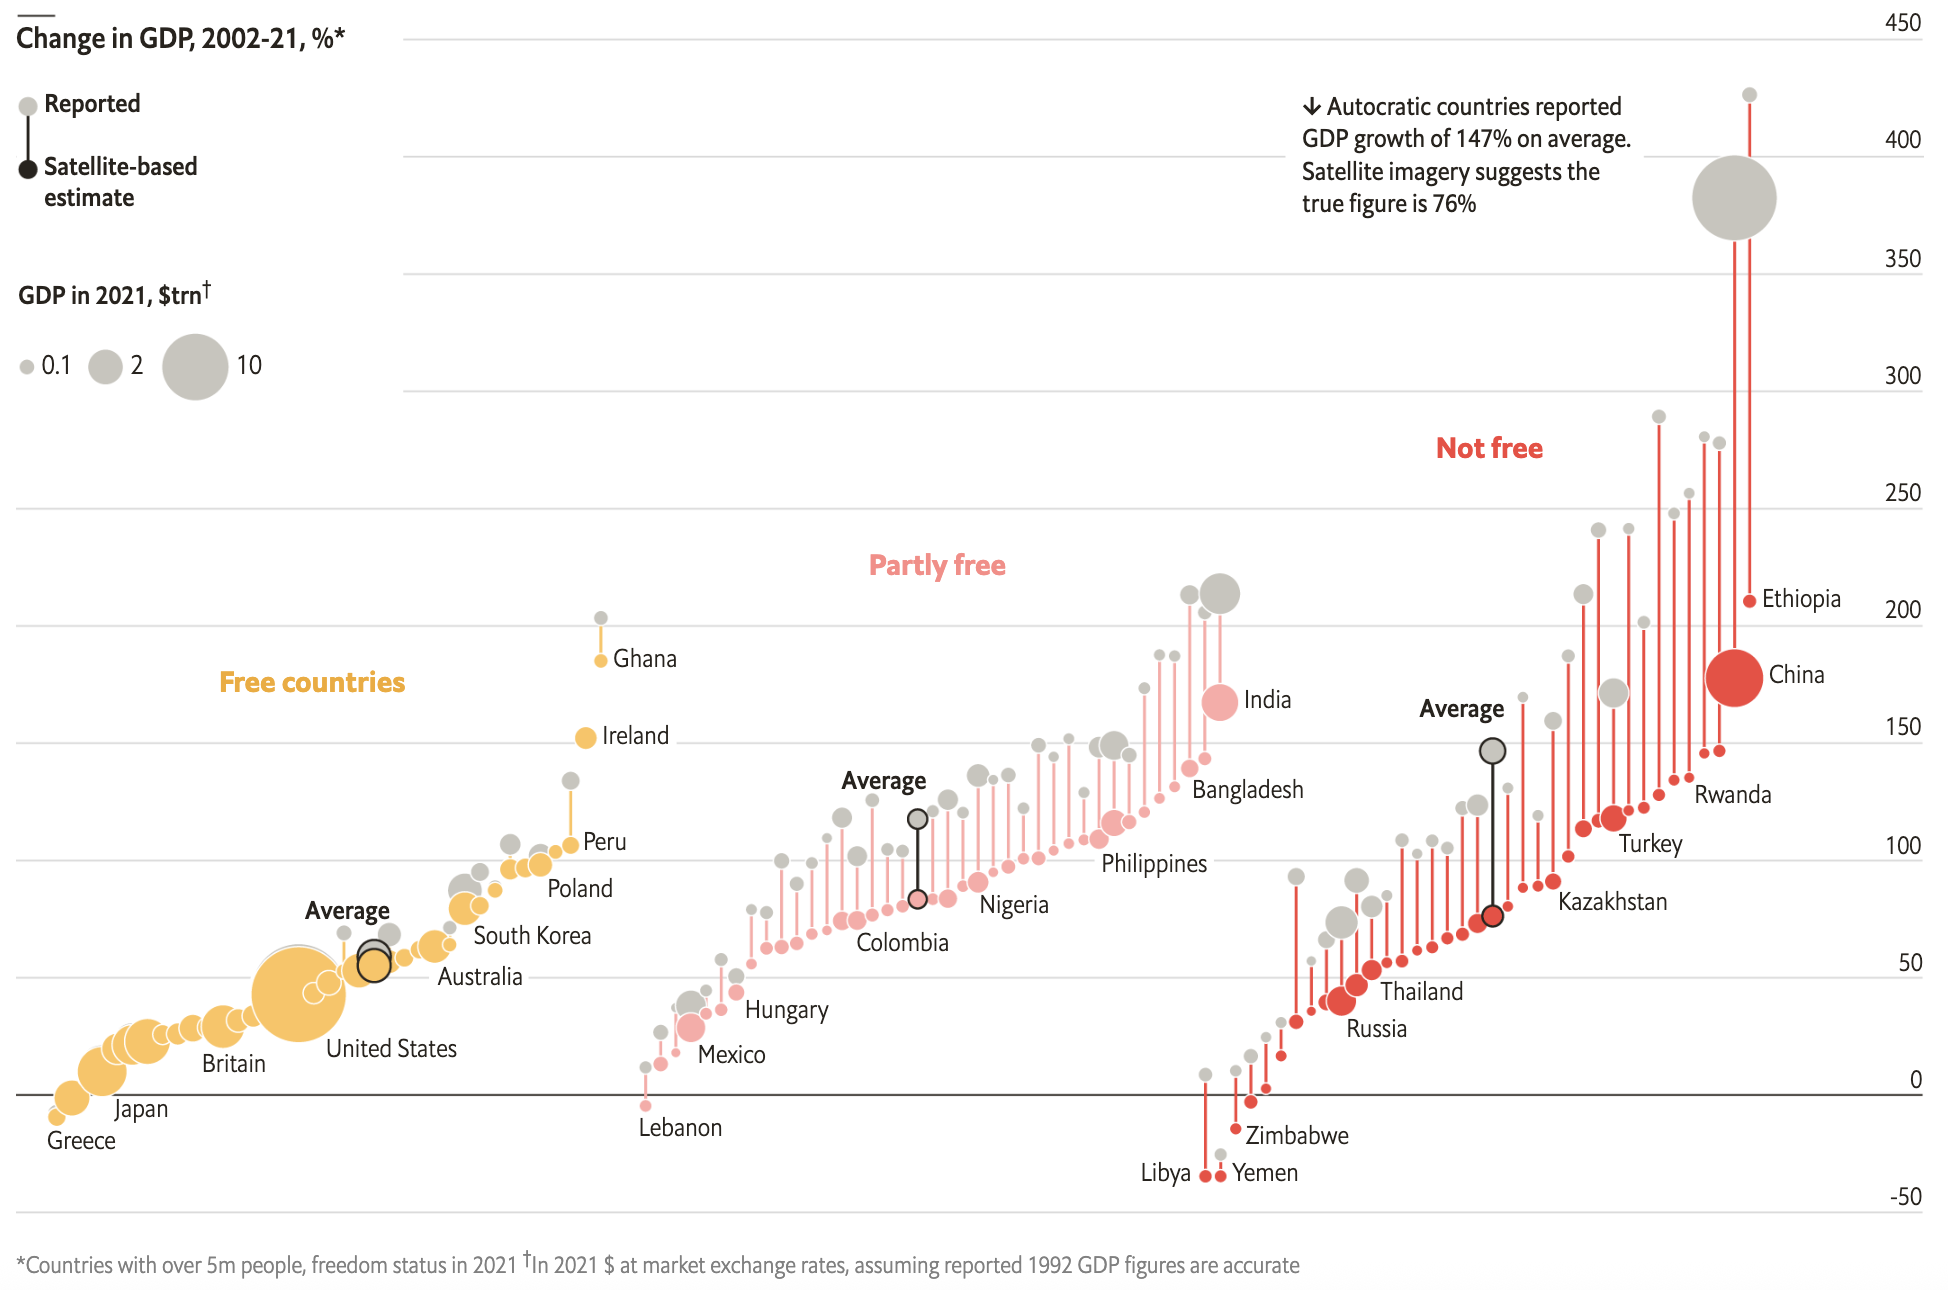
\includegraphics[height=0.8\textheight, keepaspectratio]{gdp_manipulation.png}
\end{frame}

% ============================================================================
\begin{frame}{Outline}
   \begin{enumerate}
      \setlength\itemsep{0.35cm}
      \item {\color{gray!50}Course overview and logistics}
      \item {\color{gray!50}Measuring the economy: GDP}
      \item \textbf{Comparing GDP over time}
      \item Comparing GDP across countries
      \item Beyond GDP
   \end{enumerate}
\end{frame}

% ============================================================================
\sectionframe{Comparing GDP over time}
% ============================================================================

\begin{frame}{Nominal GDP growth in Canada}
   \begin{figure}
      \centering
      
\includegraphics[width=\textwidth]{gdp_nominal_canada.png}
   \end{figure}
\end{frame}

\begin{frame}{Nominal vs.\ real GDP growth in Canada}
   \begin{figure}
      \centering
      
\includegraphics[width=\textwidth]{gdp_nominal_real_canada.png}
   \end{figure}
\end{frame}

\begin{frame}[t]{GDP and prices}
   \begin{defbox}
      \vspace{-0.5cm}
      \begin{itemize}
         \setlength\itemsep{0.15cm}
         \item \textbf{Nominal GDP} = output valued at \textit{current} prices
         \item \textbf{Real GDP} = output valued at \textit{constant} prices
         \item \textbf{GDP deflator} = $\frac{\text{Nominal GDP}}{\text{Real GDP}} \times 100$
      \end{itemize}
   \end{defbox}
   \vspace{0.05cm}
   \begin{keyinsight}
      Nominal GDP comparisons are contaminated by price changes. Real GDP isolates quantity changes, allowing us to measure true economic growth.
   \end{keyinsight}
\end{frame}

\begin{frame}[t]{What if higher prices reflect better quality?}
   \small
   When a good/service \textbf{improves}, part of the price increase reflects quality, not inflation:
   \vspace{0.15cm}
   \begin{itemize}
      \setlength\itemsep{0.15cm}
      \item \textbf{New cars:} average price rose from $\sim$\$23K (2005) to $\sim$\$48K (2024) --- but modern cars have 10+ airbags, lane assist, backup cameras, and last twice as long
      \item \textbf{Cancer drugs:} a year of treatment cost $\sim$\$10K in 2000; today's immunotherapies exceed \$100K --- but the cancer mortality rate has fallen 34\% since 1991
   \end{itemize}
   \vspace{0.1cm}
   \begin{keyinsight}
      Statistical agencies try to adjust for this (\textbf{hedonic pricing}), but actual quality growth is roughly \textbf{3$\times$ larger} than what they measure. If we overstate inflation, we understate real GDP growth\ldots
      \hfill{\scriptsize\textcolor{HECgray}{Bils \& Klenow, \textit{AER}, 2001}}
   \end{keyinsight}
\end{frame}

\begin{frame}{Inflation is back in fashion\ldots}
   \begin{tikzpicture}[remember picture, overlay]
      \setcounter{newshl}{0}
      \newsheadline[bloomberg]{Bloomberg}{``The Affordability Crisis Should Have Been Over By Now''}
      \newsheadline[washpost]{The Washington Post}{``Rising prices fueled by tariffs, delayed inflation report shows''}
      \newsheadline[globeandmail]{The Globe and Mail}{``Canada's inflation rate rises to 2.4\% as grocery prices surge''}
      \newsheadline[ledevoir]{Le Devoir}{``Vers une nouvelle hausse du prix des aliments en 2026''}
      \newsheadline[wsj]{The Wall Street Journal}{``Trump's Tariffs Cost the Average Household \$1,000 Last Year''}
      \newsheadline[lapresse]{La Presse}{``L'inflation alimentaire ne dispara\^itra pas de sit\^ot''}
   \end{tikzpicture}
\end{frame}

\begin{frame}{What is inflation?}
   \begin{defbox}[Inflation]
      The \% rate of change in the \textbf{overall price level} between two periods.
   \end{defbox}

   \begin{equation*}
      \pi_t = \frac{P_t - P_{t-1}}{P_{t-1}} = \%\Delta P \quad \text{where $P_t =$ price level at time $t$}
   \end{equation*}

   \vspace{0.3cm}

   \textbf{Key question:} how do we measure $P_t$?
   \vspace{0.2cm}
   \begin{itemize}
      \setlength\itemsep{0.15cm}
      \item \textbf{GDP deflator:} prices of all goods produced domestically (broad)
      \item \textbf{Consumer Price Index (CPI):} prices of a basket of goods bought by consumers (most commonly reported)
   \end{itemize}
\end{frame}

\begin{frame}{Recent inflation in Canada}
   \begin{figure}
      \centering
      
\includegraphics[width=0.95\textwidth, height=0.75\textheight, keepaspectratio]{inflation_cpi_deflator_canada.png}
   \end{figure}
\end{frame}

\begin{frame}{Headline vs.\ core inflation}
   \begin{figure}
      \centering
      
\includegraphics[width=0.95\textwidth, height=0.75\textheight, keepaspectratio]{inflation_headline_core_canada.png}
   \end{figure}
\end{frame}

\begin{frame}[t]{High-frequency inflation indicators}
   \small
   Scraping \textbf{millions of online prices daily}, for a real-time alternative to official CPI data
   \vspace{0.1cm}
   \begin{figure}
      \centering
      
\includegraphics[width=0.92\textwidth, height=0.75\textheight, keepaspectratio]{inflation_highfreq_cavallo.png}
   \end{figure}
\end{frame}

\begin{frame}[t]{New product bias and the price of light}
   \small
   When an entirely \textbf{new product} appears, there is no predecessor to compare it to. The price index starts fresh, missing the leap\ldots
   \vspace{0.25cm}
   \begin{keyinsight}[The price of light (Nordhaus, 1997)]
      \vspace{-0.5cm}
      \begin{itemize}
         \item What are we buying when we buy a candle, a kerosene lamp, or a light bulb?
         \item We are buying \textbf{light} --- lumens!
         \item From candles to LEDs, the true cost per lumen fell by a factor of $\sim$500.
         \item But prices don't track ``lumens'' --- they track \textbf{products} (e.g., candles, lamps).
         \item Each technology switch \textbf{resets} the comparison --- the revolution is invisible.
      \end{itemize}
   \end{keyinsight}
\end{frame}

% ============================================================================
\begin{frame}{Outline}
   \begin{enumerate}
      \setlength\itemsep{0.35cm}
      \item {\color{gray!50}Course overview and logistics}
      \item {\color{gray!50}Measuring the economy: GDP}
      \item {\color{gray!50}Comparing GDP over time}
      \item \textbf{Comparing GDP across countries}
      \item Beyond GDP
   \end{enumerate}
\end{frame}

% ============================================================================
\sectionframe{Comparing GDP across countries}
% ============================================================================

\begin{frame}{The world economy at a glance}
   \vspace{-0.2cm}
   \begin{figure}
      \centering
      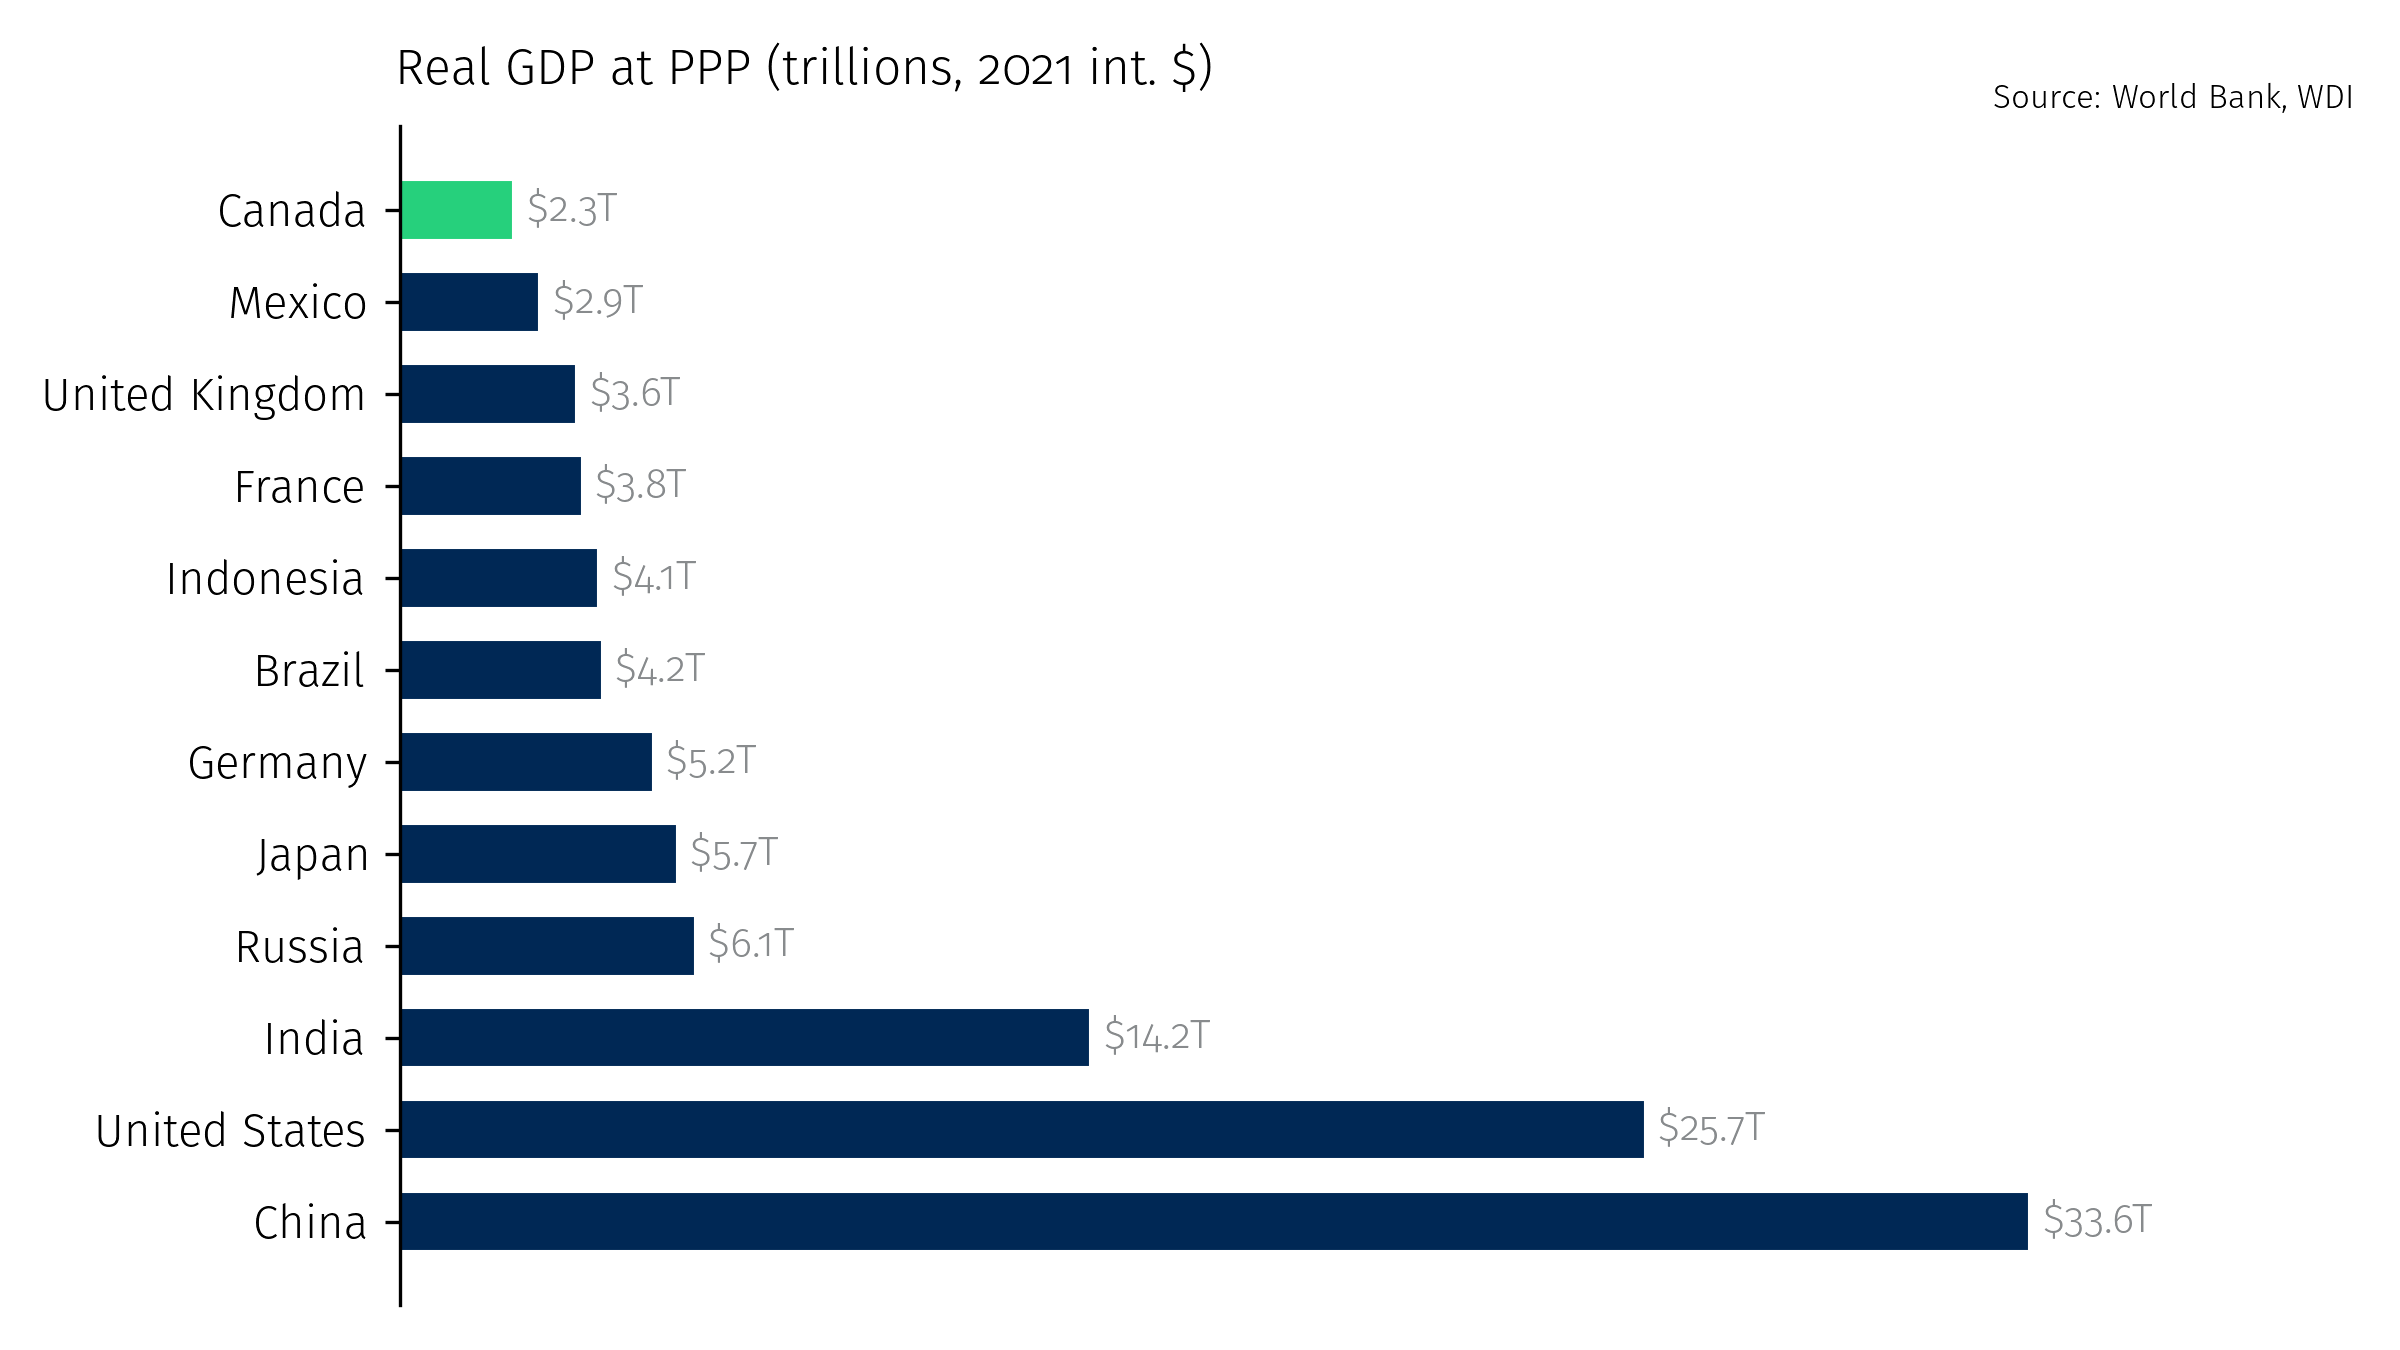
\includegraphics[width=\textwidth, height=0.75\textheight, keepaspectratio]{gdp_ppp_world.png}
   \end{figure}
   \vspace{-0.3cm}
   \footnotesize China has overtaken the US in PPP terms --- but what does ``PPP'' mean?
\end{frame}

\begin{frame}[t]{How to deal with different units?}
   \framesubtitle{Why exchange rates can be misleading}
   \small

   \textbf{Two ways to convert GDP into a common currency:}
   \vspace{0.15cm}
   \begin{enumerate}
      \setlength\itemsep{0.15cm}
      \item \textbf{Market exchange rates:}  $\smallquad e^N = \mathdollar_D / \mathdollar_F$
      \vspace{0.1cm}
      \begin{itemize}
         \setlength\itemsep{0.1cm}
         \item Widely available and updated frequently
         \item Problem: very volatile, and ignores price-level differences
      \end{itemize}
      \item \textbf{Purchasing Power Parity (PPP):} $\smallquad e^{PPP} = P_D / P_F$
      \vspace{0.1cm}
      \begin{itemize}
         \setlength\itemsep{0.1cm}
         \item Better living standards comparisons: dollar buys more in Lagos than NYC
         \item Are goods/services comparable across countries?
         \item Updated less frequently
         \item Real exchange rate: $e^R = e^N / e^{PPP}$
      \end{itemize}
   \end{enumerate}
\end{frame}

\begin{frame}{Higher prices in richer countries (Balassa-Samuelson effect)}
   \vspace{-0.2cm}
   \begin{figure}
      \centering
      
\includegraphics[width=\textwidth, height=0.8\textheight, keepaspectratio]{gdp_per_capita_vs_price_level.png}
   \end{figure}
\end{frame}

\begin{frame}[t]{The Big Mac Index}
   \small
   \vspace{-0.1cm}
   \begin{columns}[T]
      \begin{column}{0.6\textwidth}
         \begin{figure}
            \centering
            
\includegraphics[width=\textwidth, height=0.82\textheight, keepaspectratio]{big_mac_index.png}
         \end{figure}
      \end{column}
      \begin{column}{0.37\textwidth}
         A Big Mac is (roughly) the same product everywhere $\to$ ``quick and dirty'' PPP measure
         \vspace{0.2cm}

         \textbf{Example (Switzerland):}
         \vspace{0.05cm}
         \begin{itemize}
            \setlength\itemsep{0.05cm}
            \footnotesize
            \item In Switzerland: CHF 6.90
            \item In the U.S.: \$5.69
            \item Implied PPP: $\frac{6.90}{5.69} = 1.21 \text{ CHF} / \mathdollar$
            \item Market rate $\approx 0.88 \text{ CHF} / \mathdollar$
            \item CHF is \textbf{overvalued}
         \end{itemize}
         \vspace{0.15cm}
         {\footnotesize Published by \textit{The Economist} since 1986 --- half-serious, half-fun}
      \end{column}
   \end{columns}
\end{frame}

\begin{frame}[t]{Real GDP vs.\ real GDP per capita}
   \small
   \begin{itemize}
      \setlength\itemsep{0.15cm}
      \item \textbf{Real GDP} measures the total size of the economy
      \item \textbf{Real GDP per capita} measures the average standard of living
   \end{itemize}
   \vspace{0.1cm}
   \begin{bizimplication}[Market strategy]
      \small You sell luxury handbags. Should you expand to a country with high GDP or high GDP per capita? What if you sell affordable consumer goods with thin margins?
   \end{bizimplication}
   \vspace{0.1cm}
   \begin{bizimplication}[Compensation]
      \small Your Canadian employees ask for a raise because ``the economy is growing.'' GDP is up 15\% over the past decade. Is that a good argument for higher wages?
   \end{bizimplication}
\end{frame}

\begin{frame}{Canada is keeping up with the United States\ldots}
   \begin{figure}
      \centering
      
\includegraphics[width=\textwidth]{gdp_canada_usa.png}
   \end{figure}
\end{frame}

\begin{frame}{Until you account for population growth\ldots}
   \begin{figure}
      \centering
      
\includegraphics[width=\textwidth]{gdp_per_capita_canada_usa.png}
   \end{figure}
\end{frame}

\begin{frame}{GDP vs.\ GDP per capita across countries}
   \vspace{-0.2cm}
   \begin{figure}
      \centering
      
\includegraphics[width=\textwidth, height=0.78\textheight, keepaspectratio]{gdp_vs_gdp_per_capita.png}
   \end{figure}
   \vspace{-0.3cm}
   \footnotesize Large economy $\neq$ rich population. India and China have massive GDP but modest GDP per capita.
\end{frame}

% ============================================================================
\begin{frame}{Outline}
   \begin{enumerate}
      \setlength\itemsep{0.35cm}
      \item {\color{gray!50}Course overview and logistics}
      \item {\color{gray!50}Measuring the economy: GDP}
      \item {\color{gray!50}Comparing GDP over time}
      \item {\color{gray!50}Comparing GDP across countries}
      \item \textbf{Beyond GDP}
   \end{enumerate}
\end{frame}

% ============================================================================
\sectionframe{Beyond GDP}
% ============================================================================

\begin{frame}[t]{What GDP does not capture}
   \small
   GDP is a useful but incomplete measure of well-being. It misses:
   \vspace{0.1cm}
   \begin{itemize}
      \setlength\itemsep{0.1cm}
      \item \textbf{Inequality:} a country's GDP can grow while most citizens get poorer
      \item \textbf{Leisure time:} working 80h/week raises GDP, but well-being may be low
      \item \textbf{Health and well-being:} life expectancy, mental health, morbidity
      \item \textbf{Environmental degradation:} pollution, resource depletion, climate damage
      \item \textbf{Political freedom:} democracy, human rights, corruption
      \item \textbf{Safety and security:} crime rates, conflict
   \end{itemize}
   \vspace{0.05cm}
   \begin{bizimplication}[ESG and stakeholder value]
      \footnotesize Investors and consumers increasingly judge firms on dimensions GDP ignores. Understanding these limits helps anticipate where regulation and market expectations are heading.
   \end{bizimplication}
\end{frame}

\begin{frame}{}
   \small
   \begin{quotation}
      Our gross national product, now, is over \$800 billion dollars a year, but that gross national product–if we judge the United States of America by that–that gross national product counts air pollution and cigarette advertising, and ambulances to clear our highways of carnage. It counts special locks for our doors and the jails for the people who break them. It counts the destruction of the redwood and the loss of our natural wonder in chaotic sprawl. It counts napalm and counts nuclear warheads and armored cars for the police to fight the riots in our cities. It counts Whitman’s rifle and Speck’s knife, and the television programs which glorify violence in order to sell toys to our children. Yet the gross national product does not allow for the health of our children, the quality of their education or the joy of their play. It does not include the beauty of our poetry or the strength of our marriages, the intelligence of our public debate or the integrity of our public officials. It measures neither our wit nor our courage, neither our wisdom nor our learning, neither our compassion nor our devotion to our country, it measures everything in short, except that which makes life worthwhile. And it can tell us everything about America except why we are proud that we are Americans.
      \hfill{\scriptsize\textcolor{HECgray}{Robert F. Kennedy, 1968}}
   \end{quotation}
\end{frame}

\begin{frame}{Human Development Index (HDI)}
   Index developed by the UN with three ingredients:
   \vspace{0.15cm}
   \begin{itemize}
      \setlength\itemsep{0.15cm}
      \item \textbf{Health:} life expectancy at birth
      \item \textbf{Education:} mean years of schooling for adults + expected years of schooling for children
      \item \textbf{Standard of living:} GNI per capita (PPP-adjusted)
   \end{itemize}
   \vspace{0.5cm}
   What are the \textbf{pros and cons} of this index compared to GDP per capita?
   \vspace{0.15cm}
   \begin{itemize}
      \setlength\itemsep{0.15cm}
      \item Captures more dimensions of well-being, not just income
      \item Arbitrary scaling/weighting of each ingredient
   \end{itemize}
\end{frame}

\begin{frame}{HDI vs.\ GDP per capita}
   \begin{figure}
      \centering
      
\includegraphics[width=\textwidth]{hdi_vs_gdp_per_capita.png}
   \end{figure}
\end{frame}

\begin{frame}[t]{Beyond GDP: Jones and Klenow (2016)}
   \small
   \textbf{Key idea:} GDP per capita misses important dimensions of welfare
   \vspace{0.05cm}
   \begin{itemize}
      \setlength\itemsep{0.1cm}
      \item How much extra consumption needed in the U.S.\ to be as well off as in country $X$?
      \item Accounts for \textbf{consumption}, \textbf{life expectancy}, \textbf{leisure}, and \textbf{inequality}
      \item Grounded in economic theory (expected lifetime utility), not ad-hoc weighting
   \end{itemize}
   \vspace{0.1cm}
   \begin{keyinsight}[Key findings]
      \vspace{-0.5cm}
      \begin{itemize}
         \setlength\itemsep{0.1cm}
         \item Western Europe: welfare closer to U.S.\ than GDP suggests (more leisure, longer lives, less inequality)
         \item Poor countries: welfare \textit{even lower} than GDP suggests (shorter lives, higher inequality)
      \end{itemize}
   \end{keyinsight}
\end{frame}

\begin{frame}{Beyond GDP: welfare vs.\ GDP per capita}
   \begin{figure}
      \centering
      
\includegraphics[width=\textwidth]{beyond_gdp.png}
   \end{figure}
   \vspace{-0.3cm}
   \footnotesize Above the 45$^\circ$ line $\to$ welfare exceeds what GDP predicts.
   Below $\to$ welfare falls short.
\end{frame}

% ============================================================================
\sectionframe{Where are we going next?}
% ============================================================================

\begin{frame}{Connecting the themes to the course}
   \renewcommand{\arraystretch}{1.5}
   \centering
   \small
   \begin{tabular}{>{\bfseries}l l}
      \toprule
      \textbf{Theme} & \textbf{Course sessions} \\
      \midrule
      Why are some countries richer than others? & S2: Long-run economic growth \\
      What are the drivers of income inequality? & S3: The labor market \\
      Why does the economy boom and bust? & S4: Business cycles \\
      Why and how to fight against recessions? & S5: Monetary \& fiscal policy \\
      What is the future of globalization? & S6: Intl. trade \& imbalances \\
      \bottomrule
   \end{tabular}
\end{frame}

\end{document}